\documentclass[]{foi} 

\usepackage[utf8]{inputenc}
\usepackage{lipsum}

\vrstaRada{\projekt}

\title{Identificiranje korisnika pomoću dinamike tipkanja}
\predmet{\predmetSI}

\author{Karlo Vardijan, Lovro Pejaković, Filip Šoštarić, Stanko Smrček} 

\spolStudenta{\musko} 

\mentor{Bogdan Okreša Đurić}
\spolMentora{\musko} 
\titulaProfesora{dr. sc.}

\godina{2024}
\mjesec{ožujak}

\indeks{0016147086, 0016150223, 0016149647, 0016149535}

\smjer{Informacijsko i programsko inženjerstvo}


\sazetak{Dinamika tipkanja primjer je ponašajne biometrijske karakteristike koji se može koristitiu svrhu identifikacije i autentifikacije. Modernim algoritmima umjetne inteligencije, specifično strojnog i dubokog učenja, moguće je koristiti specifičnosti dinamike tipkanja korisnika u svrhu otkrivanja identiteta. Kroz praktični primjer demonstrirat će se način na koji identifikacija dinamikom tipkanja funkcionira te će se kroz analizu rezultata donjeti zaključak o korištenju spomenute biometrijske karakteristike u praksi.}
% abstract of 100 to 300 words.

\kljucneRijeci{dinamika tipkanja, biometrija, identifikacija, umjetna inteligencija, strojno učenje}
% keywords including 7 +/- 2 syntagms

\acrodef{VAS}{višeagentni sustav}



\begin{document}

\maketitle

\tableofcontents

\makeatletter \def\@dotsep{4.5} \makeatother
\pagestyle{plain}



\chapter{Uvod}

Cilj ovog projekta je analizom dinamike tipkanja identificirati korisnika. U ovom radu opisat će se sama dimanika tipkanja kao biometrijska karakteristika, u kojim područjima se primjenjuje i karakteristične mjere koje pohranjujemo te pomoću kojih na kraju vršimo samo identifikaciju. Biti će spomenuti sigurnosni rizici vezani za uporabu dinamike tipkanja i algoritmi strojnog učenja koji se koriste kod identifikacije. Detaljnije će se opisati metoda odabrana za praktični dio projekta. Na kraju slijedi opis implementiranog sustava za identifikaciju korisnika pomoću dinamike tipkanja. Analizirat će se rezultati dobiveni korištenjem implementiranog rješenja te odabranog seta podataka u svrhu identifikacije.

\chapter{Dinamika tipkanja kao biometrijska karakteristika}
Identifikacija je proces određivanja identiteta osobe bez prethodne deklaracije od strane osobe koju pokušavamo identificirati.\cite{Kasprowski2022} Identifikacija se može smatrati kao 1 naprema više veza jer iz nekog skupa korisnika pokušavamo odrediti kome pripadaju karakteristike pomoću kojih vršimo sam proces identifikacije. Značajke koje se koriste u biometriji se dijele na fizičke i ponašajne. Fizičke uključuju stvari poput otiska prsta i strukture lica dok ponašajne obuhvaćaju način hoda, glas, potpis te dinamiku tipkanja.\cite{Kasprowski2022}

Za razliku od fizičkih karakteristika koje su unikatne od osobe do osobe, ponašajne karakteristike se mijenjaju tijekom vremena te nisu toliko pouzdane što se tiče sigurnosti. Ponašajne karakteristike su obično implementirane kao potpora fizičkim. Na ponašajne karakteristike utječu stvari poput emocionalnog stanja osobe, zdravstvenih uvjeta te uvjeta okoline. Gore navedene stvari su primjenjive na dinamiku tipkanja koja je fokus ovog projekta. Obje vrste karakteristika moraju ispunjavati uvjete koje biometrijske karakteristike trebaju imati. To su jedinstvnenost, univerzalnost, lakoća prikupljanja, nepromjenjivost i prihvatljivost.\cite{Kasprowski2022} Jedinstvenost kaže da bi karakteristika trebala biti jedinstvena za osobu tj. dvije osobe nebi smjele imati identičnu mjeru neke značajke. Univerzalnost znači da bi sve osobe morale posjedovati tu značajku. Značajka bi trebala biti lako prikupljiva te se nebi trebala mijenjati kroz vrijeme. Također mora biti korisničko prihvatljiva. Sama dinamika tipkanja nije jedinstvena jer je moguće da dvije osobe tipkaju na isti način jer je to ponašajna karakteristika. Osim toga još neki problemi dinamike tipkanja su da se dinamika tipkanja može mijenjati ako smo bolesni, umorni ili ako koristimo dugačiju tipkovnicu nego inače \cite{Chang2021}. Osim ovih nedostataka dinamika tipkanja ima i dosta prednosti naprema nekim drugim biomatrijskim karakteristikama. Prednost je da netrebamo specijalne alate za prikupljanje dinamike tipkanja već korisnik tipka kao i inače,a pozadinski program skuplja podatke o tipkanju pa je zato dinamika tipkanja nenametljiva karakteristika \cite{Chang2021}. Dobar potencijal za dinamiku tipkanja je kod autetifikacije sa lozinkom u kojem dinamika tipkanja može biti drugi faktor koji se provjerava kako bi se bolje zaštitio račun korisnika jer čak ako napadač zna lozinku korisnika dinamiku tipkanja je teško lažirati. Isto tako potencijal za dinamiku tipkanja je da se nakon autentifikacije kontinuirano provjerava dinamika tipkanja korisnika i ako je drukčija nego inače može se otkritit napadač koji je uspio upasti u sustav korisnika.

Prvi primjeri korištenja dinamike tipkanja u svrhu identifikacije pojavili su se tijekom 2. Svjetskog Rata kod slanja poruka Morsovim kodom. Način na koji je poruka otipkana mogla je dati uvid u legitimnost poruke \cite{Haring2007}. U tom smislu dunamika tipkanja je relativno nova biometrijska karakteristika koja još nije puno istražena i ne postoje puno sustava koji ih koriste. 

Postojeća rješenja i implementacije bazirane su na statističkim podacima određenih događaja. Događaji koji se uglavnom koriste su duljine trajanja između pritiska i odpuštanja jedne tipke (eng. Dwell time), vrijeme koje protekne između odpuštanja jedne te pritiska druge tipke (eng. Interval), vrijeme između otpuštanja prve te odpuštanja druge tipke (eng. Up to up), vrijeme između pritiska prve tipke te pritiska druge (eng. Flight time), vrijeme između pritiska prve tipke te odpuštanja druge scenariji u kojima se koriste "Shift" i "Capslock" tipke za pisanje velikih slova i korištenje strelica za pozicioniranje u tekstu.\cite{Kasprowski2022} Manje korištene značajke uključuju i poziciju prsta na tipkama što zahtjeva korištenje kamere. Također se može promatrati i odabir prstiju koji se koristi za određene tipke za koje je također potrebna kamera. Druga klasifikacija obuhvaća metrike kao što su Down-down time, Up-down time, Up-up time te Down-up time koje jednostavno opisuju vremenski razmak između otpuštanja (Up) ili pritiska (Down) prve tipke te otpuštanja ili pritiska druge.

Kod procesa identifikacije koriste se dvije vrste tekstova: oni s definiranim brojem znakova i oni s nasumično odabranom duljinom. Prva opcija je primjenjuje u većini istraživanja koja su povezana s dinamikom tipkanja. Fokus je stavljen na odabir odgovarajućih algoritma te njihovo poboljšanje. Drugi pristup se koristi za kontinuiranu autentifikaciju.\cite{Kasprowski2022} Podaci o dinamici tipkanja se obično prikupljaju tipkovnicom, no kako su pametni mobiteli u današnje vrijeme sveprisutni, moguće je i na taj način obaviti prikupljanje. Ovdje također možemo zabilježiti točne koordinate pritiska, veličinu ekrana koju prst prekriva kod određene tipke te jačinu pritiska.\cite{Lee2018}

\begin{figure}[!h]
    \centering
    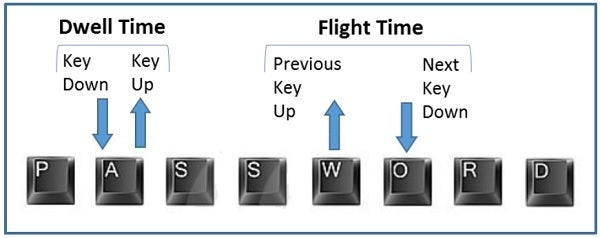
\includegraphics[width=0.6\textwidth]{slike/karakteristike.jpeg}
    \caption{Slika prikaza karakterističnih vremena dinamike tipkanja; preuzeto iz \cite{Rootstrap}}
    \label{fig:slika-kar-vremena}
\end{figure}

\chapter{Skup podataka dinamičkog tipkanja}
Za ovaj rad pronašli smo besplatni skup podataka za dinamičko tipkanje KeyRecs. Skup podataka je dobiven od 99 sudionika koji su sudjelovali u dva zadatka  \cite{Dias2023}. Prvi zadatak je bio pisanje lozinke „vpwjkeurkb“ 200 puta kroz dvije sesija, a drugi zadatak je bio prepisivanje 10 odlomaka raznih literatura isto kroz dvije sesije \cite{Dias2023}. Ti zadaci su se provodili preko web stranice koja je bilježila razna vremena tijekom tipkanja \cite{Dias2023}. Vremena koja su se bilježila su: od pritiska tipke do puštanja tipke (DU), od pritiska tipke do pritiska druge tipke (DD), od puštanja tipke do pritiska druge tipke (UD), od puštanja tipke do puštanja druge tipke(UU), od pritiska tipke do puštanja druge tipke (DU) i ukupno vrijeme tipkanja \cite{Dias2023}. Ta vremena su dobro prikazana na slici \ref{fig:graf-vremena-tipkanja}. Osim tih vremena za svakoga korisnika su  zabilježene: godine, spol, nacionalnost i dominantna ruka  \cite{Dias2023}. Podaci za prvi zadatak pisanja lozinke su zapisani kao tablica \ref{tab:KeyRecs-podaci}. U svakom redu je zabilježeno: tko je pisao, koja je sesija, koje ponavljanje i vremena za svaku tipku sifre \cite{Dias2023}. Vremena su zabilježena u kolone (D|U).tipka1.tipka2 gdje prvi dio prikazuje određeno vrijeme na temelju slike \ref{fig:graf-vremena-tipkanja} a druga dva dijela na koju tipku se odnosi \cite{Dias2023}.

\begin{table}[!h]
    \centering
    \caption{Dio podataka iz KeyRecs skupa podataka; prema \cite{Dias2023}}
    \begin{tabularx}{1\textwidth}{|l|l|l|l|l|l|l|l|l|l|}
    \hline
        \cellcolor{gray!25}participant & \cellcolor{gray!25}session & \cellcolor{gray!25}repetition & \cellcolor{gray!25}DU.v.v & \cellcolor{gray!25}DD.v.p & \cellcolor{gray!25}DU.v.p & \cellcolor{gray!25}UD.v.p & \cellcolor{gray!25}UU.v.p & \cellcolor{gray!25}DU.p.p & \cellcolor{gray!25}... \\ \hline
        p001 & 1 & 1 & 0.129 & 1.917 & 1.804 & 2.046 & 1.933 & 0.113 & ... \\ \hline
        p001 & 1 & 2 & 0.112 & 0.192 & 0.096 & 0.304 & 0.208 & 0.096 & ... \\ \hline
        p001 & 1 & 3 & 0.088 & 0.253 & 0.182 & 0.341 & 0.27 & 0.071 & ... \\ \hline
        ... & ... & ... & ... & ... & ... & ... & ... & ... & ... \\ \hline
    \end{tabularx}
    \\[10pt]
    \label{tab:KeyRecs-podaci}
\end{table}


\begin{figure}[!h]
    \centering
    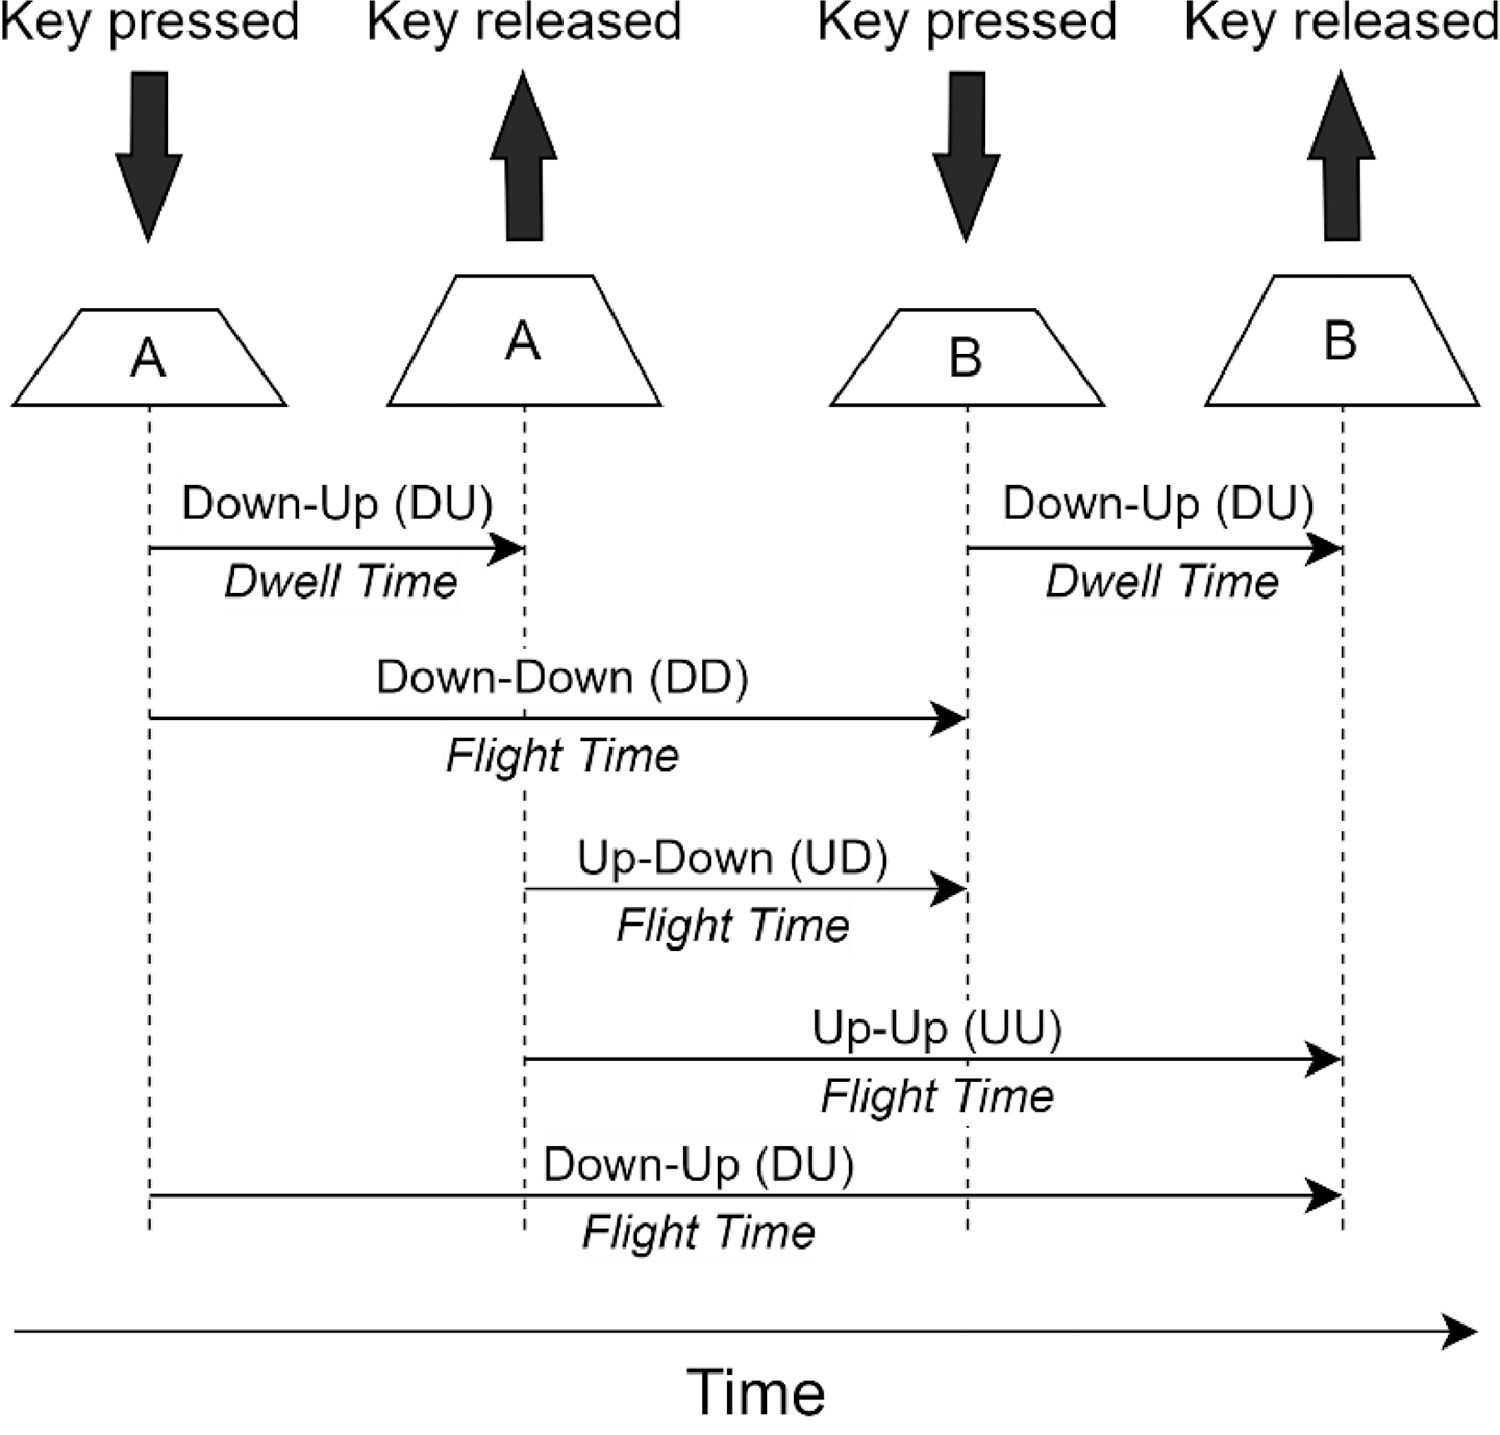
\includegraphics[width=0.6\textwidth]{slike/tipkanje-graf.jpg}
    \caption{Grafikon bilježenih vremena tijekom tipkanja; preuzeto iz \cite{Dias2023}}
    \label{fig:graf-vremena-tipkanja}
\end{figure}


\chapter{Metode analize dinamike tipkanja pomoću umjetne inteligencije}
Umjetna inteligencija je prikladan način za obradu velike količine podataka koje je potrebno obuhvatiti kako bi sa dosta velikom sigurnošću mogli autenticirati korisnika. Najčešće korištene metode su K-Nearest Neighbours (K-NN), Multi-Layer Perceptron (MLP) i Convoluted Neural Network (CNN). K-NN je neparametarski klasifikator s nadziranim učenjem. Moguće ga je koristiti za regresijski ili klasifikacijske probleme ali se tipično koristi kao klasifikacijski algoritam. Unutar klasifikacijskih problema on radi tako da se većinskim glasanjem odabire klasa koja je "najbliža" podacima danim za klasifikaciju. MLP je umjetna neuronska mreža koja se sastoji od više slojeva međusobno spojenih čvorova. Može se koristiti u regresijskim problemima i kao binaran/višeklasni klasifikator. CNN je algoritam dubokog učenja koji je prikladan za izvlačenje uzoraka iz slika \cite{Lev2024}. Najbolji algoritam za naše potrebe je K-NN algoritam pošto je jednostavan za implementirati i efektivan u klasifikaciji podataka. Istraživanja su pokazala da MLP ima malo bolje performanse od K-NN \cite{Cho2000} ali te razlike su zanemarive za potrebe ovog seminarskog rada.

\chapter{Zaključak - napiši}

Ovdje treba sažeto rezimirati najvažnije rezultate razrade teme rada. Potrebno je sažeto opisati što je predmet rada \cite{copeland2020ArtificialIntelligence}, koje su metode, tehnike, programski alati ili aplikacije korištene u razradi rada te koje su pretpostavke dokazane, a koje opovrgnute. Sadržajno, ono što se u uvodu rada najavljuje i kasnije je obuhvaćeno u samom radu, moralo bi biti opisano u zaključnom dijelu kroz rezultate rada. \cite{Kasprowski2022}


\makebackmatter

\end{document}
